\chapter{معیارهای جهش و فرآیند}
 
\label{chap:method}
با  مطالعات مروری انجام شده نقاطی از این حوزه که نیازمند پژوهش بیشتر هستند تا بتوان به وسیله‌ی آن به ارائه‌ی روشی کاراتر در پیش‌بینی خطا پرداخت مشخص شد. مقاله‌ی \cite{bowes2016mutation} اولین مقاله‌ای است که  یک  روش پیش‌بینی خطا با استفاده از تحلیل جهش ارائه نموده  است و این موضوع نیازمند تحقیق بیشتر است. از طرف دیگر بر طبق مقاله‌ی \cite{radjenovic2013software} استفاده از معیارهای فرآیند علی‌رغم توانایی بالقوه‌ای که در پیش‌بینی خطا دارند، در پژوهش‌های کمتری مورد بررسی قرار گرفته‌اند. یکی از دلایل آن می‌تواند نو ظهور بودن این معیارها نسبت به سایرین باشد. معیارهای فرآیند از جنبه‌های مختلف نیز از سایر معیار‌ها برتری دارند \cite{rahman2013and}. \\
این پایانامه قصد دارد سه رویکرد  پیشنهادی را به منظور بهبود پیش‌بینی خطا بررسی کند.  این رویکردها عبارتند از:
\begin{enumerate}
\item
معیارهای جهش و معیارهای فرآیند در کنار یکدیگر استفاده می‌شوند و به وسیله‌ی آنها پیش‌بینی انجام می گیرد. این دو دسته معیار در پژوهش‌های گذشته مطرح شده‌اند اما تاکنون در کنار یکدیگر قرار نگرفته‌اند.
\item
معیارهای جدیدی مطرح می‌شوند که مبتنی بر مفاهیم آزمون جهش و فرآیند توسعه‌ی نرم‌افزار است.
\item
معیارهای جدیدی مطرح می‌شوند که با کمک مفاهیم جهش سعی در بهبود معیارهای فرآیند دارند.
\end{enumerate}

همچنین جهت استخراج معیارها و انجام پیش‌بینی خطا در این پایانامه ابزاری به نام JPredict طراحی و ساخته می‌گردد.

\section{معیارهای جهش و فرآیند}
\label{sec:method-phase1}

این رویکرد با توجه به مقاله‌ی \cite{bowes2016mutation} مطرح شده که در آن بررسی به کارگیری معیارهای جهش و فرآیند را در پژوهش‌های آتی توصیه می‌کند.  همچنین  معیار جهش یک معیار  مرتبط با کد است. مقاله‌ی \cite{rahman2013and}  بیان می‌کند که معیارهای کد ایستا هستند و تمایل دارند که یک موجودیت را در انتشارهای متوالی حاوی خطا معرفی کنند. حال شرایطی را در نظر بگیرید که که امتیاز جهش در یک موجودیت کم باشد و دلیل آن کافی نبودن مجموعه آزمون باشد چراکه توسعه‌دهندگان از درست بودن کد اطمینان دارند یا اینکه پس از انتشارهای متوالی خطاها بر طرف شده است. چنین موجودیتی حاوی خطا نیست اما با توجه به معیار جهش خطا‌خیز است. با در نظر گرفتن معیارهای فرآیند در مورد این موجودیت که نشان می‌دهند پایدار و بدون تغییر است از میزان خطا‌خیز بودن آن کاسته می‌شود و انتظار می‌رود کارایی مدل پیش‌بینی بهبود یابد. 
برای  انجام این رویکرد مجموعه معیارهای جهش  از پژوهش \cite{bowes2016mutation}  و معیارهای فرآیند از پژوهش \cite{rahman2013and} انتخاب می‌شوند. در جداول  \ref{tab:process-metircs} و \ref{tab:mutation-metircs} معیارهای مورد نظر آورده شده است و به ترتیب در قسمت‌های \ref{subsec:metrics} و \ref{sec:mutation} معرفی شده‌اند.\\


از آنجا که  در این پایانامه پیش‌بینی‌ها در سطح پرونده انجام می‌شود، معیارها برای هر پرونده جداگانه محاسبه می‌شوند. در ادامه هر یک از معیارهای فرآیند معرفی و نحوه‌ی محاسبه‌ی آن‌ها بیان می‌شود. معیارهای جهش به طور مستقیم توسط ابزارهای موجود محاسبه‌ می‌گردد و نیازمند توضیح بیشتر نیستند.\\




%%%%%%%%%%%
\section{معیارهای جهش مبتنی بر فرآیند}
\label{sec:method-phase-two}
در رویکرد دوم، چهار معیار جدید در این پایانامه معرفی می‌شوند که با استفاده از مفاهیم آزمون جهش و تاریخچه‌ی توسعه‌ی نرم‌افزار ساخته می‌شوند. از این رو این معیارها  \نام{معیارهای جهش مبتنی بر فرآیند}{Process Based Mutation Metrics (PBMM)} نامیده شده‌اند. 

\begin{enumerate}
	\item  
	\textbf{
		تعداد جهش‌یافته‌های تولید شده‌ی جدید نسبت به انتشار قبلی برنامه: }همانطور که در مقاله‌ی \cite{just2014mutants} مطرح شده جهش‌یافته‌ها جایگزین خوبی برای خطاهای واقعی می‌باشند. زمانی که تعداد جهش‌یافته‌های جدید زیاد باشد یعنی تغییراتی که خطا‌خیز‌تر هستند بیشتر است. به منظور محاسبه‌ی این معیار لازم است خطوط اضافه شده به پرونده‌ی مورد نظر در ثبت کنونی، نسبت به انتشار قبلی مشخص شود و سپس تعداد جهش یافته‌هایی که این خطوط تولید می‌کنند شمرده شوند. 
	\item 
	\textbf{
		تعداد جهش‌یافته‌های متمایز در چند انتشار اخیر:} این معیار نشان می‌دهد موجودیت مورد بررسی به چه میزان سابقه‌ی تغییراتی را دارد که احتمال بروز خطا را افزایش می‌دهد. تعداد انتشارها باید به گونه‌ای باشد که کم یا زیاد نباشد. زیرا تعداد انتشارهای کم سبب می‌شود تفاوت چندانی با معیار قبلی نداشته باشد و سابقه‌ی تغییرات به اندازه‌ی کافی مد نظر قرار نگیرد. از طرف دیگر در نظر گرفتن تعداد زیادی انتشار، هم هزینه‌بر است و هم به دلیل تغییرات زیاد  پرونده در طول توسعه‌ی نرم‌افزار اطلاعات اولیه مفید نخواهد بود.  تعداد انتشارهای  در نظر گرفته شده در این پایانامه چهار می‌باشد. نحوه‌ی محاسبه به این شکل است که برای هر انتشار تعداد جهش‌یافته‌ها در انتشار جدید، نسبت به قبلی  شمرده می‌شود و با یکدیگر جمع زده  می‌شوند. 
	
	\item 
	\textbf{
		میزان تغییرات مثبت امتیاز جهش  در چند انتشار اخیر:}
	تغییرات امتیاز جهش نشان از تغییرات در برنامه و آزمون‌های نرم‌افزار است. این معیار نشان می‌دهد این تغییرات به چه میزان در جهت بهبود کیفیت نرم‌افزار بوده. چراکه امتیاز بالاتر جهش نشان از کیفیت بهتر آزمون‌ها و در نتیجه نرم‌افزار است.  به منظور محاسبه‌ی این معیار در هر انتشار امتیاز جهش محاسبه می‌شود و در صورتی که نسبت به انتشار قبلی تغییر مثبت  بود به مجموع تغییرات  مثبت  افزوده می‌شود. 
	\item 
	\textbf{
		میزان تغییرات منفی امتیاز جهش در چند انتشار اخیر:}
	این معیار مشابه معیار سوم عمل می‌کند با این تفاوت که میزان تغییرات در خلاف جهت بهبود نرم‌افزار را می‌سنجد. 	
	
\end{enumerate}


\section{معیارهای ترکیبی جهش-فرآیند}
رویکرد سوم با توجه به مطالب گفته شده در مقاله‌ی \cite{rahman2013and} مطرح شده که بیان می‌کند معیارها هر چقدر هم که پویا باشند (دچار رکود نشوند، مانند معیارهای فرآیند) زمانی در پیش‌بینی خطا مفید هستند که همراه با ایجاد خطا باشند. نکته‌ی قابل توجه این است که همه‌ی تغییرات در یک پرونده به یک اندازه  بر پیچیدگی پرونده نمی‌افزایند و به عبارت دیگر موجب بروز خطا نمی‌شوند. به عنوان مثال در یک پرونده به زبان جاوا ممکن است \واژه{توضیح} و یا \واژه{مستند‌جاوا} وجود داشته باشد که بروزرسانی یا اضافه و کم شدن آنها تاثیری بر روند اجرای برنامه و میران پیچیدگی ندارند با این حال در محاسبه‌ی معیارهای پیش‌بینی خطا در نظر گرفته می‌شوند. هدف از ارائه‌ی معیارهای \نام{ترکیبی جهش-فرآیند}{Process-Mutation Hybrid} بهبود کاستی‌های معیارهای فرآیند در چنین شرایطی است. در اینجا دو معیار \موکد{مقدار نرمال شده‌ی خطوط اضافه شده} و یا \موکد{کم شده}  جهت اصلاح انتخاب شده‌اند.  این دو معیار جز شاخص‌ترین معیارهای فرآیند هستند.\\
در نگاه اول  این ایده به ذهن می‌رسد که با توجه به تعداد جهش‌یافته‌هایی که  اضافه   کردن  خط ایجاد می‌کند و یا حذف هر خط  از بین می‌برد. اضافه یا کم شدن خطوط وزن دهی شود و به منظور اجرای آن از دو  فرمول زیر بهره گرفت.\\
\begin{latin}
	
	$M_1 =\ number\ of\ lines\ added\ \times \ number\ of\ muatants\ derived$\\
	
	$M_2 =\ number\ of\ lines\ deleted\ \times \ number\ of\ mutants\ derived$\\
\end{latin}


با وجود مناسب بودن ایده ی اولیه با بررسی‌های بیشتر دو مشکل در معیارهای فوق مشخص می‌شود.\\
مشکل اول : هدف از ارئه ی این معیارها وزن دهی به خطوط اضافه و کم شده است. نکته قابل توجه این است که هر خط باید به صورت جداگانه وزن دهی شود و وزن یک خط بر وزن خط دیگر تأثیری نداشته باشد. مثال زیر را در نظر بگیرید.
\begin{latin}
\flushleft
//this method is important  \emph{→ 0 mutant} \\
// this method get root of \emph{→ 0 mutant}\\
// sum of a plus b \emph{→ 0 mutant} \\ 
b = sqrt(a+b) \emph{→ 2 mutant} \\
\end{latin}

فرض کنید ۴ خط بالا به یک پرونده اضافه شده است. معیار  \موکد{مقدار نرمال شده‌ي خطوط اضافه شده} قبل از نرمال سازی عدد چهار را نمایش می‌دهد در حالی که از این چهار خط ۳ خط توضیح است. حال معیار اولیه پیشنهادی برابر ۸ خواهد بود که بدیهی است، از هدف ارايه ی معیار فاصله گرفته است. حال اگر تنها جهش یافته‌های تولید شده در خطوط اضافه شده را در نظر بگیریم این مقدار می‌تواند جایگزین مناسبی باشد. در‌ واقع نگاشتی  ارائه می‌شود که هر خط از برنامه را به یک عدد نگاشت می‌دهد. این عدد میزان پیچیدگی آن خط و یا احتمال بروز خطا را تعریف می‌کند.  لازم به یادآوری است که در مقاله‌ی  \cite{just2014mutants} اشاره شده که جهش یافته ها جایگزین خوبی برای خطاهای واقعی هستند. این نگاشت برابر است با تعداد جهش یافته های تولید شده در آن خط.

مشکل دوم: این معیار برای عملکرد هرچه بهتر مشابه معیار  \موکد{مقدار نرمال شده‌ی خطوط اضافه شده}‌ نیاز به نرمال‌سازی دارد. به جهت نرمال‌سازی نمی‌توان از همان روش استفاده کنیم چراکه در آن وزن‌دهی به خطوط وجود ندارد و از آن مهم‌تر توضیحات را نیز در نظر می‌گیرد. از طرف دیگر این امکان وجود ندارد که برای تمام خطوط اضافه یا کم شده در کل پروژه در طول یک انتشار جهش یافته تولید شود (به دلیل زمانبر بودن و پیچیدگی‌های فراوان در پیاده‌سازی). در مقاله‌ی \cite{bird2011don} اشاره شده که تعداد ثبت‌ها می‌تواند نشانگر میزان تغییرات باشد. بنابرین از تعداد ثبت‌های کل پروژه در طول یک انتشار به منظور نرمال‌سازی استفاده خواهد شد.

\section{JPredict}
جهت آگاهی از عملکرد معیارهای مطرح شده لازم است این معیارها استخراج شوند با استفاده از آنها مدل پیش‌بینی ساخته شود و با یکدیگر مقایسه شوند. جهت انجام این وظایف ابزار  در این پایانامه ابزار JPredict ارائه گردیده است که می‌تواند این وظایف را به صورت خودکار انجام دهد. همچنین قابلیت گسترش جهت کار با انواع مجموعه‌داده‌ها و استخراج معیارهای تعریف شده‌ی جدید توسط کاربر را دارد. 

نمای کلی از فرآیند‌هایی که در ابزار Jpredict انجام می‌گیرد در شکل \ref{fig:jpredict-process}  آمده است. این شکل نشان می‌دهد که در ابتدا انواع مختلفی از اطلاعات لازم است که از منابع متفاوت بدست آید. ابتدا اطلاعات پرونده‌های حاوی خطا از گزارش‌های خطا بیرون بدست می‌آید. این گزارش‌ها می‌توانند داده‌های موجود در سیستم ردگیری خطا و یا  مجموعه‌داده‌ی مرتبط با خطاهای پروژه‌های نرم‌افزاری باشد. همچنین تعدادی از پرونده‌های بدون نیز انتخاب می‌شوند. این انتخاب به صورت تصادفی انجام می‌شود و بسته به خواست کاربر محدودیت‌هایی در انتخاب در نظر گرفته می‌شود. اطلاعات این دو نوع پرونده با استفاده از سامانه‌ی کنترل نسخه تکمیل می‌گردد و در پایگاه داده ذخیره می‌شود. نوع دیگری از اطلاعات که از سامانه‌ی کنترل نسخه استخراج می‌شود اطلاعات تاریخی مربوط به توسعه‌ی پروژه‌ی نرم‌افزاری است. این اطلاعات بسته به معیارهایی که قرار است از آنها استخراج شود می‌تواند برای تمامی پرونده‌های موجود در سامانه‌ی کنترل نسخه استخراج شود و یا تنها برای پرونده‌های حاوی خطا و سالم انتخاب شده. معمولا در صورتی که استخراج اطلاعات پرهزینه باشد تنها برای پرونده‌های انتخابی اطلاعات تاریخی استخراج می‌شود. 

از آنجا که معیارهای جهش نیز باید محاسبه شوند لازم است تا برای پرونده‌های انتخابی کد منبع پروژه‌ی  مرتبط از سامانه‌ی کنترل نسخه بازیابی شود سپس با استفاده از یکی از ابزارهای جهش بر روی  پرونده تحلیل جهش انجام می‌گیرد. این دسته از اطلاعات  نیز در پایگاه‌داده ذخیره می‌شود. 

معیارهای مورد نظر با استفاده \واژه{پرسمان} مناسب از اطلاعات موجود در پایگاه داده استخراج می‌شوند و از آنها در ساخت مدل پیش‌بینی استفاده می‌گردد. مدل پیش‌بینی نمونه‌ی جدید را دریافت می‌کند و سالم یا خطادار بودن آنرا پیش‌بینی خواهد کرد. در واقع این نمونه یک بردار ویژگی از معیارهای استفاده شده در ساخت مدل است. در نهایت  با توجه به نتایج مدل ساخته شده ارزیابی می‌گردد.

\begin{figure}[H]
	\centering
	\includegraphics[width=1.0\textwidth]{img/method/jpredict-process.png}
	\caption{ نمایی کلی از فرآیند‌های موجود در JPredict}
	\label{fig:jpredict-process}
\end{figure}

\subsection{ساختار Jpredict}
واحدهای اصلی تشکیل دهنده‌ی Jpredict در شکل \ref{fig:jpredict-module} نشان داده شده‌ است. واحد Mutation وظیفه‌ی تولید جهش و انجام تحلیل را بر عهده دارد و در واقع رابط میان Jpredict و ابزار  خارجی آزمون جهش می‌باشد. واحد Repository ارتباط با سامانه‌ی کنترل نسخه‌ی پروژه‌های مورد آزمایش را بر عهده دارند. اطلاعات لازم را بازیابی می‌کند و کد منبع ثبت‌های مختلف را در مسیری قرار می‌دهد تا ابزار جهش با آن کار کند. واحد BugReport اطلاعات پرونده‌های حاوی خطا را از منبع بیرونی دریافت می‌کند و با استفاده از واحد Repository آنها را تکمیل می‌کند.  انتخاب پرونده‌های سالم نیز بر عهده‌ی این واحد می‌باشد. واحد MutationMetric دستورات مرتب با جهش به واحد Mutation می‌دهد و نتایج اولیه را در پایگاه داده ذخیره می‌کند و با اجرای پرسمان مناسب معیارها را محاسبه می‌نماید. واحد ProcessMetric نیز  از داده‌هایی که واحد Reposiotry بر روی پایگاه داده ذخیره کرده است استفاده می‌کند و معیارهای فرآیند را محاسبه می‌کند. واحد DataBase وظیفه‌ی ارتباط با پایگاه داده‌ را دارد و همچنین حاوی پرسمان‌های مختلف است. در ادامه به بررسی جزیی‌تر هریک از واحدها پرداخته می‌شود.


\begin{figure}[H]
	\centering
	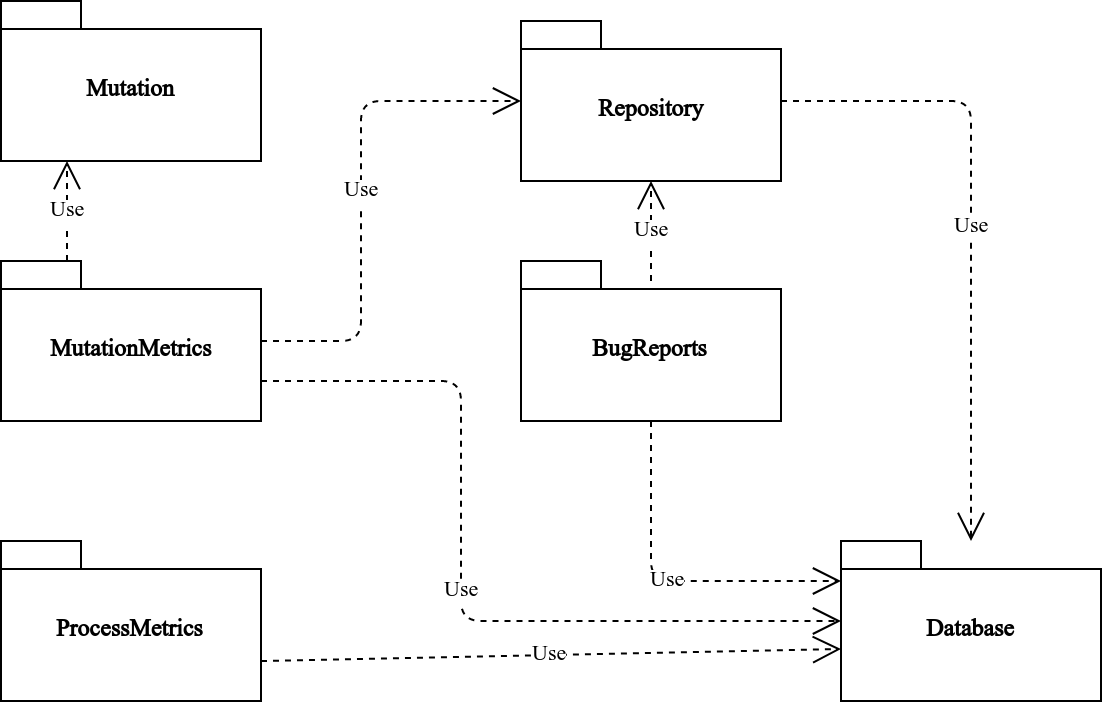
\includegraphics[width=.8\textwidth]{img/method/component-jpredict.png}
	\caption{ نمایی از واحدهای تشکیل دهنده‌ی JPredict}
	\label{fig:jpredict-module}
\end{figure}

\subsection{واحد  Repository}
 
همانطور که اشاره شد این واحد دو وظیفه‌ی اصلی دارد: استخراج اطلاعات از سامانه‌ی کنترل نسخه و دریافت کد منبع برای یک پروژه‌ی خاص. 

با توجه به مرور معیارهای استفاده شده در پژوهش‌های پیشین که در قسمت \ref{subsec:metrics}‌معرفی شدند و معیارهای انتخاب شده در قسمت \ref{sec:method-phase1}  لازم است اطلاعات زیر استخراج گردد.
\begin{itemize}
\item
اطلاعات ثبت‌های مختلف در پروژه شامل شماره‌ی ثبت در سامانه‌ی کنترل نسخه، نام ثبت‌کننده، پرونده‌های تغییر یافته در ثبت، تعداد خطوط حذف و اضافه شده
\item
انتشار قبلی ثبت‌ها
\item
مشارکت‌کنندگان در یک پرونده در زمان ثبت و میزان مشارکت آنها

\end{itemize}

پس از استخراج هر یک از این اطلاعات لازم است آنها به نحو مناسبی در پایگاه داده قرار گیرند. این واحد چهار جدول در پایگاه داده می‌سازد که در زیر مشخص شده‌اند:
\begin{itemize}
\item CommitInfo :
حاوی اطلاعات ثبت‌ها
\item CommitChangedFiles : 
حاوی اطلاعات پرونده‌های تغییر یافته در هر ثبت نسبت به ثبت قبلی
\item ProjectRelease :
انتشارهای موجود در پروژه‌ها
\item Participation :
مشارکت کنندگان در پرونده و میزان مشارکت آنها به تفکیک ثبت
\end{itemize}

وظیفه‌ی دیگر این واحد بازیابی کد منبع  پروژه در یک ثبت خاص  می‌باشد.  جهت انجام این امر،  برای هر سامانه‌ی کنترل نسخه لازم است از کتابخانه‌ی مناسب با آن کمک گرفته شود. یکی دیگر از وظایف این سامانه مشخص کردن تفاوت میان دو ثبت از پروژه است. از این قابلیت هم در مشخص کردن تعداد خطوط کم و اضافه شده در جدول CommitChangedFiles استفاده می‌شود و هم در محاسبه‌ی معیارهای ارائه شده‌ی جدید. 

\subsection{واحد ProcessMetrics}
معیارهای فرآیند در جدول متناظری ذخیره می‌شوند که  این جدول قبل از محاسبه‌ی معیارها مقداردهی اولیه می‌شود . هر سطر از این جدول به یکی از پرونده‌هایی که لازم است معیارها برای آن محاسبه شود اختصاص می‌یابد. این امر سبب می‌شود محاسبه‌ی هر معیار مستقل از دیگر انجام گیرد و امکان بروزرسانی داشته باشد. نحوه‌ی محاسبه‌ی یک معیار فرآیند در واحد ProcessMetrics در شکل \ref{fig:process-chart}  آمده است. در این فرآیند ابتدا اطلاعات پرونده‌ها از پایگاه داده بازیابی می‌گردد. سپس برای هر پرونده شئ مربوط به آن که حاوی معیارهای فرآیند است بازیابی می‌گردد. این شئ معادل یک سطر از جدول حاوی معیارهای فرآیند در پایگاه داده است. سپس لازم است که یک یا چند پرسمان تکمیل شود. این پرسمان‌ها از قبل در واحد Database  قرار دارند که نیازمند تکمیل هستند. پس از تکمیل آنها به واحد Database داده می‌شوند تا اجرا شوند. در صورت نیاز محاسبات بیشتری بر روی نتایج پرسمان انجام می‌گیرد. در نهایت شئ حاوی معیارهای فرآیند بروزرسانی می‌شود. 

به منظور محاسبه‌ی معیار فرآیند یک کلاس انتزاعی در نظر گرفته شده است که شامل مراحل نشان داده شده در شکل \ref{fig:process-chart}  است. هر معیار به طور جداگانه گسترشی از این کلاس خواهد بود که  قسمت‌های انتزاعی را پیاده‌سازی می‌کند. بدین ترتیب امکان افزودن معیار جدید فراهم می‌گردد. 
\begin{figure}[H]
	\centering
	\includegraphics[width=.8\textwidth]{img/method/process-chart.png}
	\caption{ فرآیند محاسبه‌ی یک معیار فرآیند در Jpredict}
	\label{fig:process-chart}
\end{figure}


\subsection{واحد BugReports  }
این واحد با منبع خارجی ارتباط برقرار می‌کند و اطلاعات پرونده‌های حاوی خطا را دریافت می‌کند. همچنین بر طبق محدودیت‌های از پیش تعیین شده تعدادی فایل سالم را از پروژه در یک ثبت خاص انتخاب کند. این انتخاب می‌تواند به صورت تصادفی انجام پذیرد و فایل‌های سالم نیز توسط منبع خارجی مشخص شود. سپس به کمک واحد Repository اطلاعات پرونده تکمیل می‌گردد و در پایگاه داده ذخیره می‌شود. اطلاعات مربوط به پرونده‌های حاوی خطا در جدول BugInfo و پرونده‌های سالم در جدول CleanInfo  قرار می‌گیرد. اطلاعاتی که در این دو جدول وجود دارد عبارتند از :
\begin{itemize}
	\item 
	نام پرونده‌ی حاوی خطا
	\item
	شماره‌ی خطا (در صورتی که یک خطا بیش از چند پرونده را شامل می‌شود)
	\item
	شماره‌ی ثبتی که در آن در پرونده‌ی مورد نظر خطا رخ داده
	\item
	نام انتشار قبلی
	\item
	شماره‌ی ثبت انتشار قبلی
	\item 
	نام پروژه (در حالتی که اطلاعات خطای چندید پروژه‌ی مختلف وجود دارد)
\end{itemize}

\subsection{واحد Major}

